\documentclass{article}\usepackage[]{graphicx}\usepackage[]{color}
% maxwidth is the original width if it is less than linewidth
% otherwise use linewidth (to make sure the graphics do not exceed the margin)
\makeatletter
\def\maxwidth{ %
  \ifdim\Gin@nat@width>\linewidth
    \linewidth
  \else
    \Gin@nat@width
  \fi
}
\makeatother

\definecolor{fgcolor}{rgb}{0.345, 0.345, 0.345}
\newcommand{\hlnum}[1]{\textcolor[rgb]{0.686,0.059,0.569}{#1}}%
\newcommand{\hlstr}[1]{\textcolor[rgb]{0.192,0.494,0.8}{#1}}%
\newcommand{\hlcom}[1]{\textcolor[rgb]{0.678,0.584,0.686}{\textit{#1}}}%
\newcommand{\hlopt}[1]{\textcolor[rgb]{0,0,0}{#1}}%
\newcommand{\hlstd}[1]{\textcolor[rgb]{0.345,0.345,0.345}{#1}}%
\newcommand{\hlkwa}[1]{\textcolor[rgb]{0.161,0.373,0.58}{\textbf{#1}}}%
\newcommand{\hlkwb}[1]{\textcolor[rgb]{0.69,0.353,0.396}{#1}}%
\newcommand{\hlkwc}[1]{\textcolor[rgb]{0.333,0.667,0.333}{#1}}%
\newcommand{\hlkwd}[1]{\textcolor[rgb]{0.737,0.353,0.396}{\textbf{#1}}}%
\let\hlipl\hlkwb

\usepackage{framed}
\makeatletter
\newenvironment{kframe}{%
 \def\at@end@of@kframe{}%
 \ifinner\ifhmode%
  \def\at@end@of@kframe{\end{minipage}}%
  \begin{minipage}{\columnwidth}%
 \fi\fi%
 \def\FrameCommand##1{\hskip\@totalleftmargin \hskip-\fboxsep
 \colorbox{shadecolor}{##1}\hskip-\fboxsep
     % There is no \\@totalrightmargin, so:
     \hskip-\linewidth \hskip-\@totalleftmargin \hskip\columnwidth}%
 \MakeFramed {\advance\hsize-\width
   \@totalleftmargin\z@ \linewidth\hsize
   \@setminipage}}%
 {\par\unskip\endMakeFramed%
 \at@end@of@kframe}
\makeatother

\definecolor{shadecolor}{rgb}{.97, .97, .97}
\definecolor{messagecolor}{rgb}{0, 0, 0}
\definecolor{warningcolor}{rgb}{1, 0, 1}
\definecolor{errorcolor}{rgb}{1, 0, 0}
\newenvironment{knitrout}{}{} % an empty environment to be redefined in TeX

\usepackage{alltt}

\usepackage{float}

% Set the margins on the page to not be so large
\addtolength{\oddsidemargin}{-.875in}
\addtolength{\evensidemargin}{-.875in}
\addtolength{\textwidth}{1.75in}
\addtolength{\topmargin}{-.875in}
\addtolength{\textheight}{1.75in}

% Take off page numbering
\pagenumbering{gobble}
\IfFileExists{upquote.sty}{\usepackage{upquote}}{}
\begin{document}

\title{%
  Stat 5100 Handout 2.6.1 - R: Inference with Multiple Predictors \\
  \smallskip
  \large Stat 5100: Dr. Bean
}
\date{}

\maketitle

\textbf{Example: } (Table 7.1) Study seeks to relate (in females) amount of body fat ($Y$) to triceps skinfold thickness ($X_1$), thigh circumference ($X_2$), and midarm circumference ($X_3$).  Amount of body fat is expensive to measure, requiring immersion of person in water.  This expense motivates the desire for a predictive model based on these inexpensive predictors.

Q1: Do thigh and midarm both have no effect on body fat when triceps is in the model?

Q2: Do the relationships among the predictors cause any problems in the fitted model?

\begin{knitrout}
\definecolor{shadecolor}{rgb}{0.969, 0.969, 0.969}\color{fgcolor}\begin{kframe}
\begin{alltt}
\hlcom{# Make output easier to read by disabling scientific notation}
\hlkwd{options}\hlstd{(}\hlkwc{scipen} \hlstd{=} \hlnum{999}\hlstd{)}

\hlcom{# Input data and take a look at the first few observations}
\hlkwd{library}\hlstd{(stat5100)}
\hlkwd{data}\hlstd{(bodyfat)}
\hlkwd{head}\hlstd{(bodyfat)}
\end{alltt}
\begin{verbatim}
##   triceps thigh midarm body
## 1    19.5  43.1   29.1 11.9
## 2    24.7  49.8   28.2 22.8
## 3    30.7  51.9   37.0 18.7
## 4    29.8  54.3   31.1 20.1
## 5    19.1  42.2   30.9 12.9
## 6    25.6  53.9   23.7 21.7
\end{verbatim}
\begin{alltt}
\hlcom{# Look at the correlation matrix}
\hlkwd{cor}\hlstd{(bodyfat)}
\end{alltt}
\begin{verbatim}
##           triceps     thigh    midarm      body
## triceps 1.0000000 0.9238425 0.4577772 0.8432654
## thigh   0.9238425 1.0000000 0.0846675 0.8780896
## midarm  0.4577772 0.0846675 1.0000000 0.1424440
## body    0.8432654 0.8780896 0.1424440 1.0000000
\end{verbatim}
\begin{alltt}
\hlcom{# Look at the scatterplot}
\hlkwd{pairs}\hlstd{(} \hlopt{~} \hlstd{body} \hlopt{+} \hlstd{triceps} \hlopt{+} \hlstd{thigh} \hlopt{+} \hlstd{midarm,} \hlkwc{data} \hlstd{= bodyfat,}
       \hlkwc{main} \hlstd{=} \hlstr{"Bodyfat Data"}\hlstd{)}
\end{alltt}
\end{kframe}

{\centering 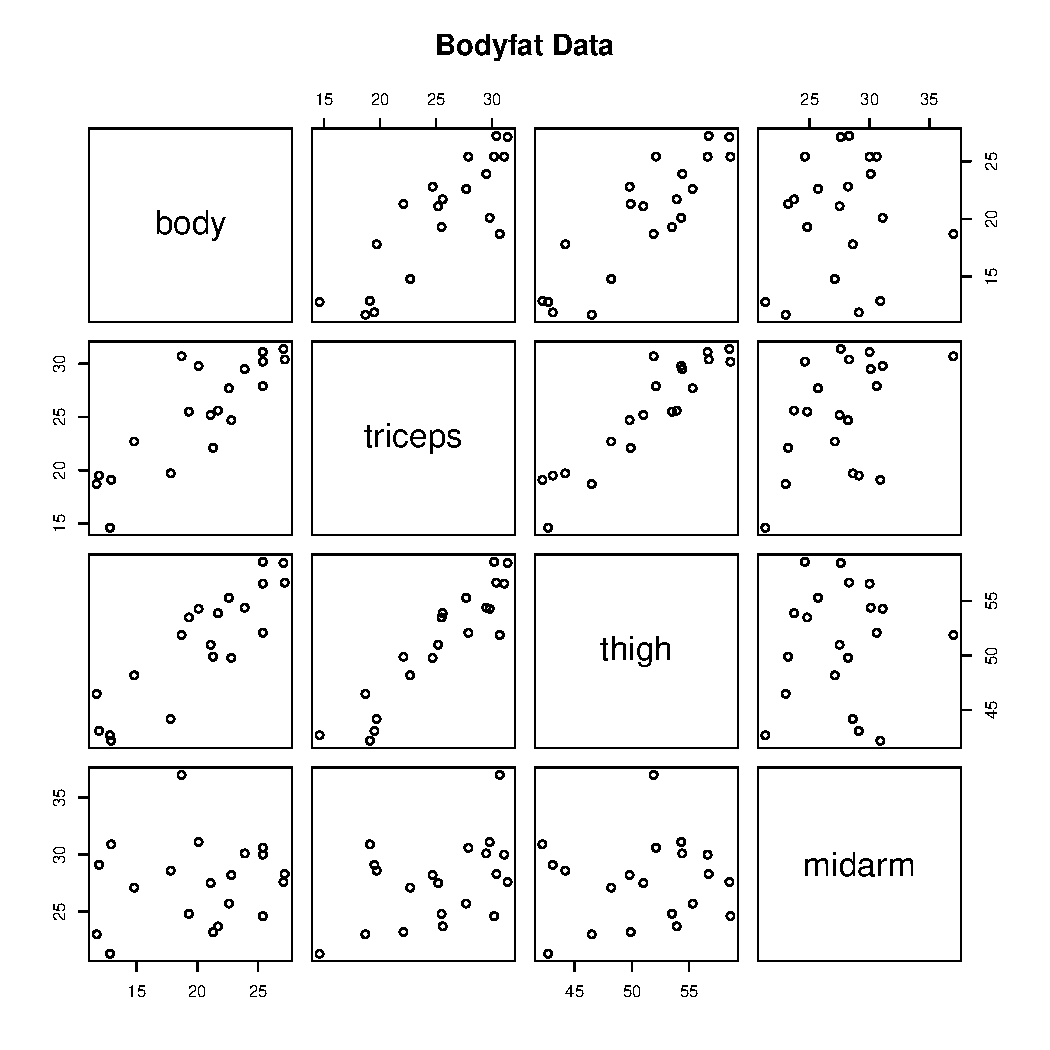
\includegraphics[width=0.6\textwidth]{figure/unnamed-chunk-1-1} 

}



\end{knitrout}

\medskip
\hrule
\medskip

\subsection*{Question 1: Test whether thigh and midarm BOTH have no effect on body when triceps is in the model}

\begin{knitrout}
\definecolor{shadecolor}{rgb}{0.969, 0.969, 0.969}\color{fgcolor}\begin{kframe}
\begin{alltt}
\hlstd{bodyfat_lm_full} \hlkwb{<-} \hlkwd{lm}\hlstd{(body} \hlopt{~} \hlstd{triceps} \hlopt{+} \hlstd{thigh} \hlopt{+} \hlstd{midarm,} \hlkwc{data} \hlstd{= bodyfat)}
\hlkwd{anova}\hlstd{(bodyfat_lm_full)}
\end{alltt}
\begin{verbatim}
## Analysis of Variance Table
## 
## Response: body
##           Df Sum Sq Mean Sq F value      Pr(>F)    
## triceps    1 352.27  352.27 57.2768 0.000001131 ***
## thigh      1  33.17   33.17  5.3931     0.03373 *  
## midarm     1  11.55   11.55  1.8773     0.18956    
## Residuals 16  98.40    6.15                        
## ---
## Signif. codes:  0 '***' 0.001 '**' 0.01 '*' 0.05 '.' 0.1 ' ' 1
\end{verbatim}
\begin{alltt}
\hlstd{bodyfat_lm_reduced} \hlkwb{<-} \hlkwd{lm}\hlstd{(body} \hlopt{~} \hlstd{triceps,} \hlkwc{data} \hlstd{= bodyfat)}
\hlkwd{anova}\hlstd{(bodyfat_lm_reduced)}
\end{alltt}
\begin{verbatim}
## Analysis of Variance Table
## 
## Response: body
##           Df Sum Sq Mean Sq F value      Pr(>F)    
## triceps    1 352.27  352.27  44.305 0.000003024 ***
## Residuals 18 143.12    7.95                        
## ---
## Signif. codes:  0 '***' 0.001 '**' 0.01 '*' 0.05 '.' 0.1 ' ' 1
\end{verbatim}
\end{kframe}
\end{knitrout}

\subsubsection*{Perform the subset F-test by hand}
\begin{knitrout}
\definecolor{shadecolor}{rgb}{0.969, 0.969, 0.969}\color{fgcolor}\begin{kframe}
\begin{alltt}
\hlcom{# (All these values are grabbed from the ANOVA tables above)}
\hlstd{SSE_Reduced} \hlkwb{<-} \hlnum{143.12}               \hlcom{# Sum of squared error for reduced model}
\hlstd{SSE_Full} \hlkwb{<-} \hlnum{98.40}                   \hlcom{# Sum of squared error for full model}
\hlstd{MSE_Full} \hlkwb{<-} \hlnum{6.15}                    \hlcom{# Mean square error for full model}
\hlstd{MSR} \hlkwb{<-} \hlstd{(SSE_Reduced} \hlopt{-} \hlstd{SSE_Full)} \hlopt{/} \hlnum{2} \hlcom{# Mean square reduction}
\hlstd{F_statistic} \hlkwb{<-} \hlstd{MSR} \hlopt{/} \hlstd{MSE_Full}
\hlstd{F_statistic}
\end{alltt}
\begin{verbatim}
## [1] 3.635772
\end{verbatim}
\begin{alltt}
\hlcom{# The F-statistic above follows a F(2,16) distribution (16 denominator degrees}
\hlcom{# of freedom because MSE_Full is calculated by SSE_Full / 16)}
\hlstd{pvalue} \hlkwb{<-} \hlkwd{pf}\hlstd{(F_statistic,} \hlnum{2}\hlstd{,} \hlnum{16}\hlstd{,} \hlkwc{lower.tail} \hlstd{=} \hlnum{FALSE}\hlstd{)}
\hlstd{pvalue}
\end{alltt}
\begin{verbatim}
## [1] 0.04992961
\end{verbatim}
\end{kframe}
\end{knitrout}

\subsubsection*{Perform the subset F-test automatically}
\begin{knitrout}
\definecolor{shadecolor}{rgb}{0.969, 0.969, 0.969}\color{fgcolor}\begin{kframe}
\begin{alltt}
\hlcom{# This is a test for the null hypothesis that thigh = midarm= 0}
\hlstd{bodyfat_lm_full} \hlkwb{<-} \hlkwd{lm}\hlstd{(body} \hlopt{~} \hlstd{triceps} \hlopt{+} \hlstd{thigh} \hlopt{+} \hlstd{midarm,} \hlkwc{data} \hlstd{= bodyfat)}
\hlstd{bodyfat_lm_reduced} \hlkwb{<-} \hlkwd{lm}\hlstd{(body} \hlopt{~} \hlstd{triceps,} \hlkwc{data} \hlstd{= bodyfat)}

\hlkwd{anova}\hlstd{(bodyfat_lm_full, bodyfat_lm_reduced)}
\end{alltt}
\begin{verbatim}
## Analysis of Variance Table
## 
## Model 1: body ~ triceps + thigh + midarm
## Model 2: body ~ triceps
##   Res.Df     RSS Df Sum of Sq      F  Pr(>F)  
## 1     16  98.405                              
## 2     18 143.120 -2   -44.715 3.6352 0.04995 *
## ---
## Signif. codes:  0 '***' 0.001 '**' 0.01 '*' 0.05 '.' 0.1 ' ' 1
\end{verbatim}
\begin{alltt}
\hlcom{# Notice here that we get the same F-statistic and p-value as we did when}
\hlcom{# we tested by hand.}
\end{alltt}
\end{kframe}
\end{knitrout}

\medskip
\hrule
\medskip

\subsection*{Question 2: Investigate the effect of relationships among predictors}

\begin{knitrout}
\definecolor{shadecolor}{rgb}{0.969, 0.969, 0.969}\color{fgcolor}\begin{kframe}
\begin{alltt}
\hlcom{# Standardize the variables and create a standardized regression model}
\hlstd{bodyfat_standardized} \hlkwb{<-} \hlkwd{data.frame}\hlstd{(}\hlkwd{scale}\hlstd{(bodyfat))}
\hlstd{bodyfat_s_lm}\hlkwb{<-} \hlkwd{lm}\hlstd{(body} \hlopt{~} \hlstd{triceps} \hlopt{+} \hlstd{thigh} \hlopt{+} \hlstd{midarm,} \hlkwc{data} \hlstd{= bodyfat_standardized)}
\hlkwd{summary}\hlstd{(bodyfat_s_lm)}
\end{alltt}
\begin{verbatim}
## 
## Call:
## lm(formula = body ~ triceps + thigh + midarm, data = bodyfat_standardized)
## 
## Residuals:
##      Min       1Q   Median       3Q      Max 
## -0.72976 -0.31552  0.07683  0.28702  0.80837 
## 
## Coefficients:
##                           Estimate             Std. Error t value Pr(>|t|)
## (Intercept) -0.0000000000000009096  0.1086017313054759154   0.000    1.000
## triceps      4.2637045669999400488  2.9665382148454386702   1.437    0.170
## thigh       -2.9287006520636991169  2.6469556563935556781  -1.106    0.285
## midarm      -1.5614167939150791486  1.1396021351584755266  -1.370    0.190
## 
## Residual standard error: 0.4857 on 16 degrees of freedom
## Multiple R-squared:  0.8014,	Adjusted R-squared:  0.7641 
## F-statistic: 21.52 on 3 and 16 DF,  p-value: 0.000007343
\end{verbatim}
\begin{alltt}
\hlcom{# Test for multicollinearity}
\hlstd{olsrr}\hlopt{::}\hlkwd{ols_coll_diag}\hlstd{(bodyfat_lm_full)}
\end{alltt}
\begin{verbatim}
## Tolerance and Variance Inflation Factor
## ---------------------------------------
##   Variables   Tolerance      VIF
## 1   triceps 0.001410750 708.8429
## 2     thigh 0.001771971 564.3434
## 3    midarm 0.009559681 104.6060
## 
## 
## Eigenvalue and Condition Index
## ------------------------------
##       Eigenvalue Condition Index      intercept        triceps          thigh
## 1 3.967956738483         1.00000 0.000001946679 0.000003196101 0.000001104251
## 2 0.020522792222        13.90482 0.000371520161 0.001319092929 0.000032620187
## 3 0.011511821361        18.56570 0.000599149515 0.000218746554 0.000325502370
## 4 0.000008647934       677.37207 0.999027383645 0.998458964415 0.999640773192
##           midarm
## 1 0.000009798156
## 2 0.001388740360
## 3 0.006933507626
## 4 0.991667953858
\end{verbatim}
\end{kframe}
\end{knitrout}



\end{document}
